\documentclass[10pt]{article}
\usepackage{listings}
\usepackage{float}
%\usepackage{svg}
\usepackage{algorithm}
\usepackage{algorithmic}
%\usepackage[]{algorithm2e}
\usepackage[superscript,biblabel]{cite}
\usepackage{graphicx}
\usepackage{subcaption}
\usepackage{fancyhdr}
\pagestyle{fancy}
%\lhead{CS7642 Reinforcement Learning 2018 Spring}
%\chead{ID: rchen350}
%\rhead{Assignment 3: Unsupervised Learning}
\fancyhead{} % clear all header fields
\fancyhead[L]{\fontsize{10}{12} \selectfont CS7641 Reinforcement Learning \\ 2018 Summer}
\fancyhead[C]{\fontsize{10}{12} \selectfont ID: rchen350 \\}
\fancyhead[R]{\fontsize{10}{12} \selectfont Project 2: Lunar Lander \\ \burl{https://github.gatech.edu/rchen350/cs7642summer2018p2}}

\lfoot{}
\cfoot{\thepage}
\rfoot{}
\renewcommand{\headrulewidth}{0.4pt}
\renewcommand{\headwidth}{\textwidth}
\renewcommand{\footrulewidth}{0pt}
%\usepackage{nips_2017}
\usepackage[utf8]{inputenc} % allow utf-8 input
\usepackage[T1]{fontenc}    % use 8-bit T1 fonts
\usepackage{hyperref}       % hyperlinks
\usepackage{url}            % simple URL typesetting
\usepackage{booktabs}       % professional-quality tables
\usepackage{amsfonts}       % blackboard math symbols
\usepackage{nicefrac}       % compact symbols for 1/2, etc.
\usepackage{microtype}      % microtypography
\usepackage{amsmath}
\DeclareMathOperator*{\argmax}{argmax} % thin space, limits underneath in displays
\DeclareMathOperator*{\argmin}{argmin} % thin space, limits underneath in displays
\DeclareMathOperator{\sgn}{sgn}
%\DeclareMathOperator*{\max}{max} % thin space, limits underneath in displays
%\DeclareMathOperator*{\min}{min} % thin space, limits underneath in displays
\usepackage{amssymb}
\usepackage{hyperref}
\usepackage{breakurl}
\usepackage[
			headheight=48pt, % height for the header block
			]{geometry}
\geometry{letterpaper, portrait, margin=1in}
\setlength\parindent{24pt}

\author{Ran Chen \\ email: ranchen@gatech.edu\vspace{-2ex}}
\title{\vspace{-1.8cm}Project 2: Lunar Lander}
\date{}
\begin{document}
\maketitle
\thispagestyle{fancy}


\begin{abstract}
This report presents a solution to the LunarLander-v2 problem provided by OpenAI Gym (\burl{https://gym.openai.com/envs/LunarLander-v2/}) using deep reinforcement learning methods. Code used to run experiments described in this report is hosted here: \burl{https://github.gatech.edu/rchen350/cs7642summer2018p2}, which is also linked in the header as required
\end{abstract}

\section{Game: LunarLander-v2} \label{game}

\textit{Game} The game is comprised of a 2D Newtonian mechanical environment, a small rocket is initialized at the top middle position of the 2D environment, with certain random but bounded initial state. The state vector of the rocket is $S=\{x_1, x_2, \dot{x_1}, \dot{x_2}, \theta, \dot{\theta}, L, R\}$, where $x_1$, $x_2$, are location coordinates in the 2D environment, and $\theta$ is the 2D rotational angle of the rocket, their first order derivatives are the velocities respectively. $L$ and $R$ are binary values indicating whether the rocket's left or right leg is touching the ground. The actions space is discrete, comprised of \{\textit{firing left engine, firing right engine, firing main engine, do nothing}\}. An episode finishes if the lander crashes or comes to rest, receiving additional $-100$ or $+100$ points respectively. Each leg ground contact is worth $+10$ points. Firing main engine incurs a $-0.3$ point penalty for each occurrence. And the goal is to land the rocket within designated location marked by two flags and maximize the total reward.\par
\bigbreak
\noindent
\textit{Approach} The Lunar Lander game can be formalized as an Markov decision process (MDP), in which, given any state vector $S$, an action $a$ needs to be chosen. Clearly this can be solved using Q-learning, where policies are generated based on Q function values for a particular state action pair $Q(S,a)$. Since this game has a large and continuous state space, the naturally suitable solution would be using function approximation to model the Q-function $Q(S,a)$, also because little information is known on what type of function this might be, it would be ideal to use an artificial neural net (ANN) to model it. In this paper, deep Q-networks (DQN)\cite{MnihPlayingAtariDeep2013, RoderickImplementingDeepQNetwork2017} are built using PyTorch as part of a Q learning process for solving this game. 






%%%%%%%%%%%%%%%%%%%figure here v
\begin{figure}[h!]
  \centering
  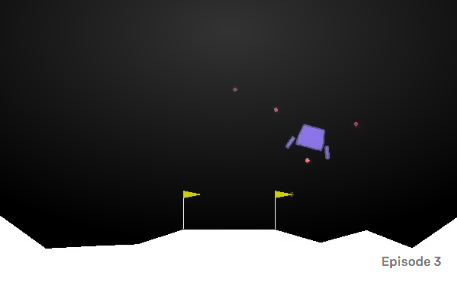
\includegraphics[width=0.45\linewidth]{illustration.png}
    \caption{An illustration of the LunarLander-v2 environment from \burl{https://gym.openai.com/envs/LunarLander-v2/}.}
  \label{fig:lunarlander}
\end{figure}
%%%%%%%%%%%%%%%%%%% figure here ^


\section{Experiments and Results} \label{experiments}
Experiments were run with different algorithms and/or different hyperparameters on the LunarLander game. The training sessions were performed until the rolling average of reward over 100 episode reach 215, and capped at total 2500 episodes. The testing of the trained networks were run 100 times, and the rewards were plotted. 3 different ANNs were tested and the network used in DQN is with 3 hidden layers and 80 nodes each.

\par

%%%%%%%%%%%%%%%%%%%figure here v

%%%%%%%%%%%%%%%%%%% figure here ^


\subsection{Experiment 1} \label{experiment1}
First, deep Q networks (DQN) is tested. Here DQN refers to bare-bone DQN with fixed targets and experience replay.\cite{MnihPlayingAtariDeep2013, RoderickImplementingDeepQNetwork2017} \par
\noindent

\begin{algorithm}
\caption{DQN with fixed Q-targets and experience replay}
\begin{algorithmic}
\STATE input: $D$ - empty replay buffer; $\theta$ - eval network parameters, $\theta^-$ - copy of $\theta$ (target network parameters)
\STATE input : $N_r$ - replay buffer maximum size; $N_b$ - training batch size; $N^-$ - target network replacement freq
\REPEAT
\STATE reset game: $S\leftarrow env()$
\STATE $R\leftarrow 0$
\FOR{$t\in \{0,1,...\}$}
\STATE generate action using $\epsilon$-greedy policy $a=\pi(S)$, observe new state from env: $\{S',r\} = env(S,a)$
\STATE add $\{S,a,r,S'\}$ to $D$, bump oldest memory from $D$ if $|D|> N_r$
\STATE sample a minibatch of $N_b$ tuples $\{S,a,r,S'\}$, construct eval and target Q values for each of $N_b$ tuples:
\STATE $Q_{\text{eval}}=Q(S,a;\theta)$ and $Q_{\text{target}}=\left\{
\begin{array}{lr}
             r & \text{if $S'$ is terminal} \\
             r+\gamma \max_{a'}(Q(S',a';\theta^-)) & \text{otherwise.}
\end{array}
\right.
$
\STATE one step optimization on $\theta$ with loss $\lVert Q_{\text{target}}-Q_{\text{eval}}\rVert$
\STATE $R\leftarrow R+r$
\STATE $\theta^- \leftarrow \theta$ if $t\mod N^- = 0$
\ENDFOR
\UNTIL{no significant improvement in $R$}
\end{algorithmic}
\end{algorithm}

As shown in \textbf{Fig} \ref{fig:train_param_0057}, with the right combination of hyperparameters ($\alpha=5\times 10^{-5}$, $\gamma=0.99$, and target net is update every 500 optimizations to the eval net). The rolling average (green line) comes close to convergence when $\epsilon$ falls below 0.2. The testing result (\textbf{Fig} \ref{fig:test_param_0057}) is also satisfactory, scoring 219 on average. However the learning curve demonstrated certain degree of instability after convergence. According to literature, using "soft updates", i.e. incrementally updating target network every time eval net is optimized, could help stabilize the learning curve by avoiding making drastic changes to target networks when outlier samples are incurred.



%%%%%%%%%%%%%%%%%%%figure here v
\begin{figure}[H]
  \centering
  \begin{subfigure}[b]{0.49\linewidth}
  \centering
  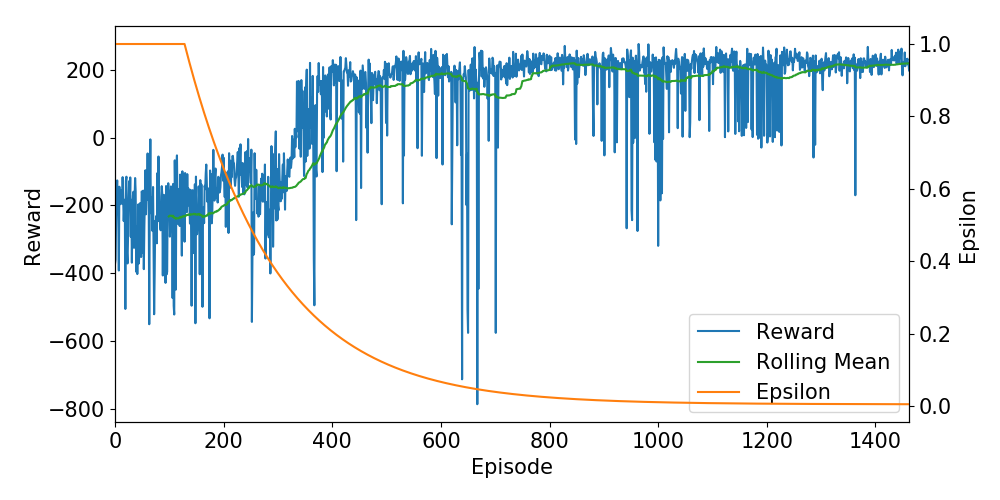
\includegraphics[width=\linewidth]{../logs/train_param_0057.png}
      \caption{}
  \label{fig:train_param_0057}
  \end{subfigure}
  \begin{subfigure}[b]{0.49\linewidth}
  \centering
  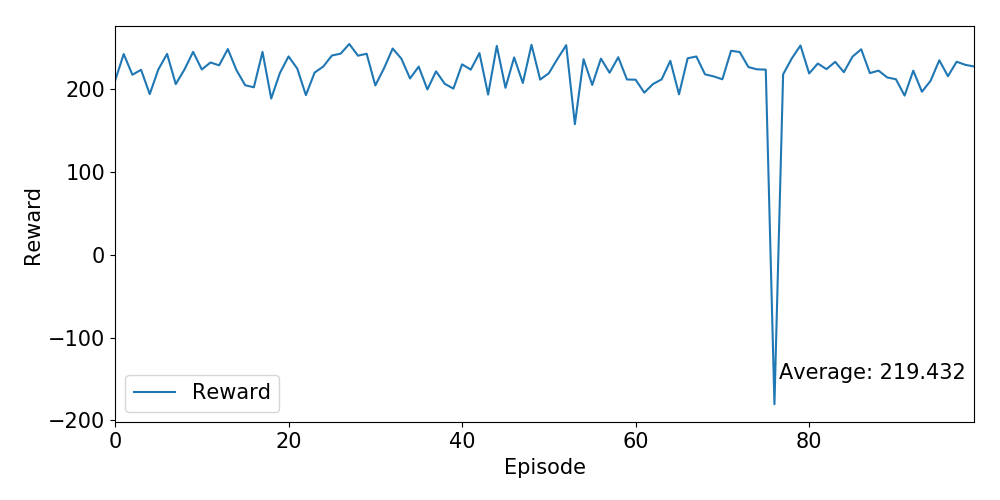
\includegraphics[width=\linewidth]{../logs/test_param_0057.png}
      \caption{}
  \label{fig:test_param_0057}
  \end{subfigure}
  \caption{DQN with fixed Q-targets (updating interval: 500): earning curve (a) and testing result (b)}
  \label{fig:param_0057}
\end{figure}

%%%%%%%%%%%%%%%%%%% figure here ^

Here the optimal learning rate ($\alpha=5\times 10^{-5}$) was obtained by experimenting. Nearby values was also tested for performance. As shown in \textbf{Fig} \ref{fig:train_param_0051} ($\alpha=2.5\times 10^{-4}$) and \ref{fig:train_param_0045} ($\alpha=2\times 10^{-4}$), the results indicate that large learning rate tends to generate extremely unstable learning curve, although for many episodes, the learning reward can reach above 200. Further changing $\alpha$ away from optimal seems deteriorate the performance more significantly, as shown in \textbf{Fig} \ref{fig:train_param_0082} ($\alpha=5\times 10^{-2}$) and \ref{fig:train_param_0083} ($\alpha=5\times 10^{-6}$), the agent is not learning anything in those situations and hardly reaching any positive reward.

%%%%%%%%%%%%%%%%%%%figure here v
\begin{figure}[H]
  \centering
  \begin{subfigure}[b]{0.49\linewidth}
  \centering
  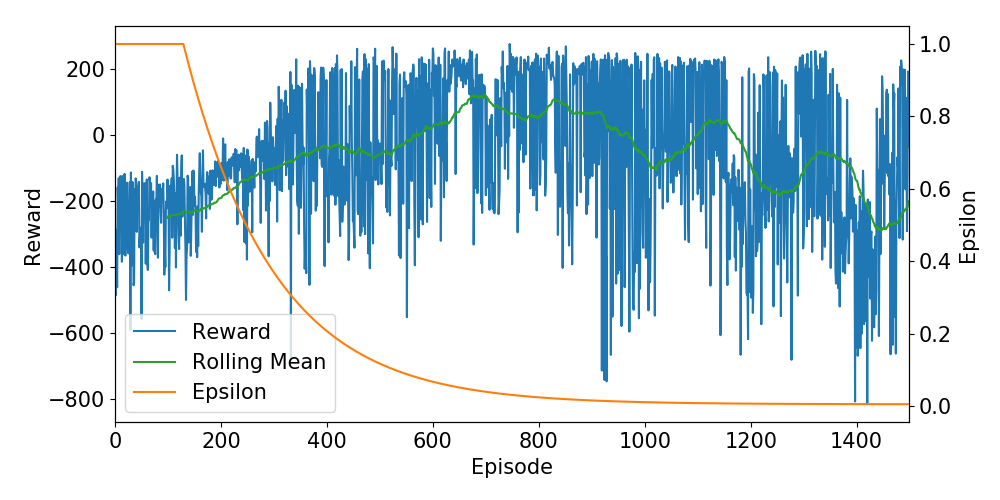
\includegraphics[width=\linewidth]{../logs/train_param_0051.png}
      \caption{}
  \label{fig:train_param_0051}
  \end{subfigure}
  \begin{subfigure}[b]{0.49\linewidth}
  \centering
  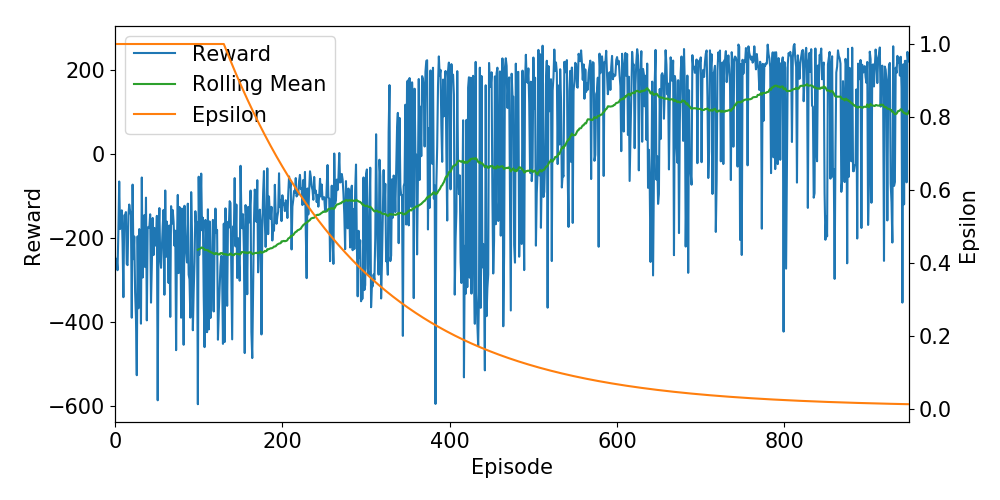
\includegraphics[width=\linewidth]{../logs/train_param_0045.png}
      \caption{}
  \label{fig:train_param_0045}
  \end{subfigure}
  \begin{subfigure}[b]{0.49\linewidth}
  \centering
  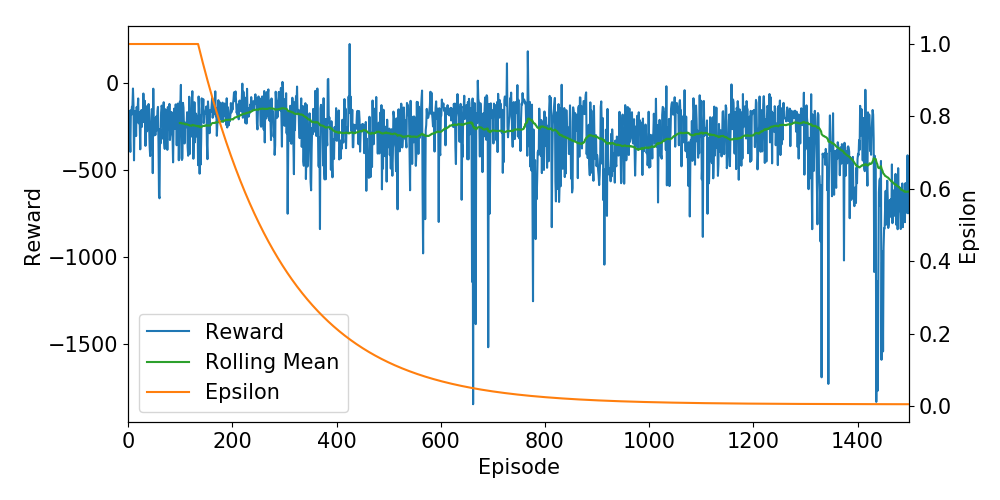
\includegraphics[width=\linewidth]{../logs/train_param_0082.png}
      \caption{}
  \label{fig:train_param_0082}
  \end{subfigure}
  \begin{subfigure}[b]{0.49\linewidth}
  \centering
  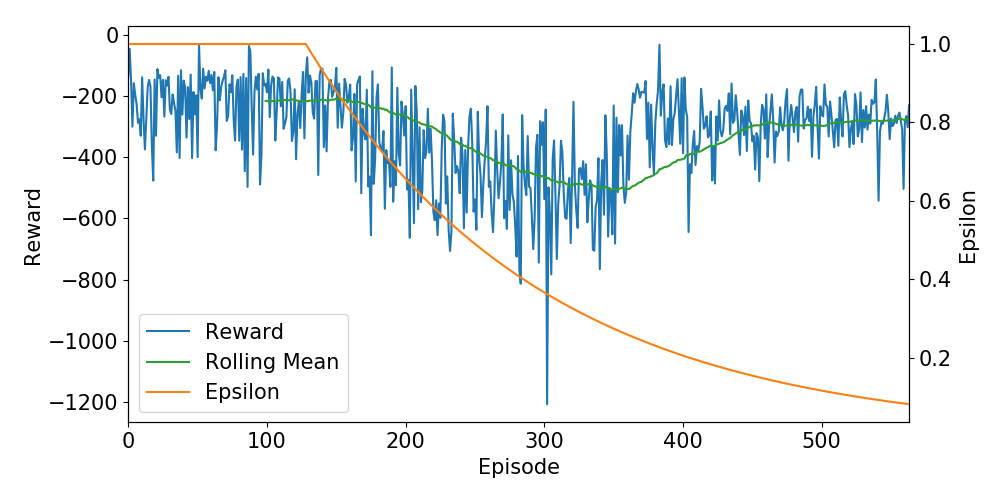
\includegraphics[width=\linewidth]{../logs/train_param_0083.png}
      \caption{}
  \label{fig:train_param_0083}
  \end{subfigure}
  \caption{DQN with fixed Q-targets (updating interval: 500): $\alpha=2.5\times 10^{-4}$ (a),  $\alpha=2\times 10^{-4}$ (b), $\alpha=5\times 10^{-2}$ (c), and $\alpha=5\times 10^{-6}$ (d).}
  \label{fig:param_0000}
\end{figure}

%%%%%%%%%%%%%%%%%%% figure here ^

\subsection{Experiment 2} \label{experiment2}
Now we replace fixed Q-targets which updates target network every 500 optimizations to eval network with a new strategy called "soft update", which update target network every time the eval network is optimized, but only by a fraction. Namely the update to target network is replaced by $\theta^- \leftarrow (1-\tau)\theta^- + \tau\theta$, instead of $\theta^- \leftarrow \theta$ if $t\mod N^- = 0$.\cite{LillicrapContinuouscontroldeep2015}\par



DQN with "soft update" ($\tau=0.02$) generated much more stable learning curve compared to fixed Q-targets (\textbf{Fig} \ref{fig:train_param_0058}) and converged as early as around episode 650. This algorithm also achieved better testing score at 227 on average (\textbf{Fig} \ref{fig:test_param_0058}).

%%%%%%%%%%%%%%%%%%%figure here v
\begin{figure}[H]
  \centering
  \begin{subfigure}[b]{0.49\linewidth}
  \centering
  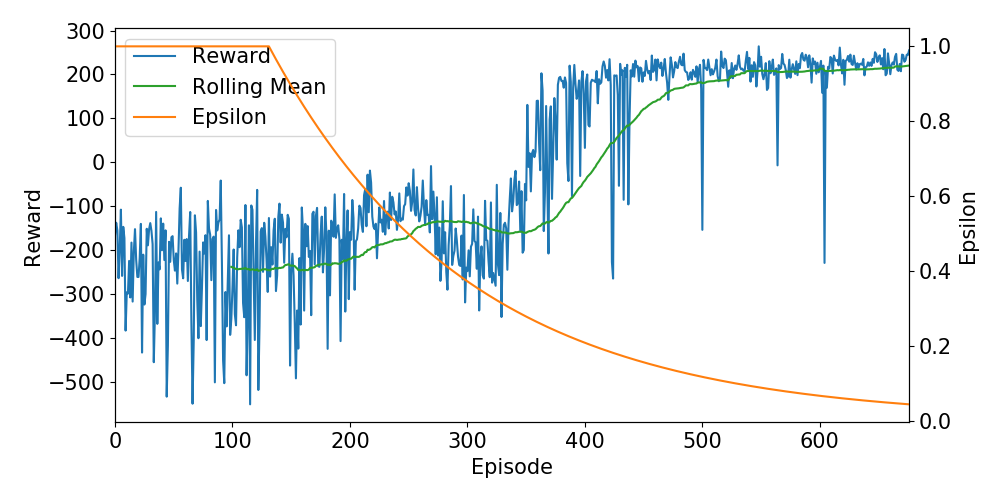
\includegraphics[width=\linewidth]{../logs/train_param_0058.png}
      \caption{}
  \label{fig:train_param_0058}
  \end{subfigure}
  \begin{subfigure}[b]{0.49\linewidth}
  \centering
  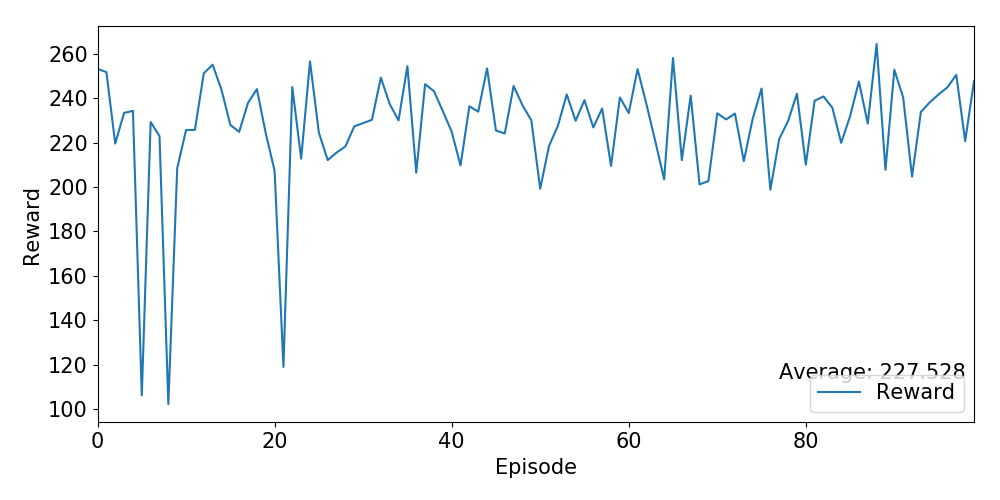
\includegraphics[width=\linewidth]{../logs/test_param_0058.png}
      \caption{}
  \label{fig:test_param_0058}
  \end{subfigure}
  \caption{DQN with "soft update" ($\tau=0.02$): learning curve (a) and testing result (b)}
  \label{fig:param_0058}
\end{figure}

%%%%%%%%%%%%%%%%%%% figure here ^
The most import hyperparameter for soft updated DQN is $\tau$ which determines how much the target network is updated by the eval network. Too large or too small update could both cause the two networks to drift away, resulting in increased loss, and in turn lead to instability in learning curves. As shown in \textbf{Fig} \ref{fig:train_param_0059} and \ref{fig:train_param_0060}, when $\tau=0.01$ and $\tau=0.05$ the learning curves were less stable and required more episodes to converge, although the testing results are both still satisfactory, scoring 210 and 219 on average respectively.

%%%%%%%%%%%%%%%%%%%figure here v
\begin{figure}[H]
  \centering
  \begin{subfigure}[b]{0.49\linewidth}
  \centering
  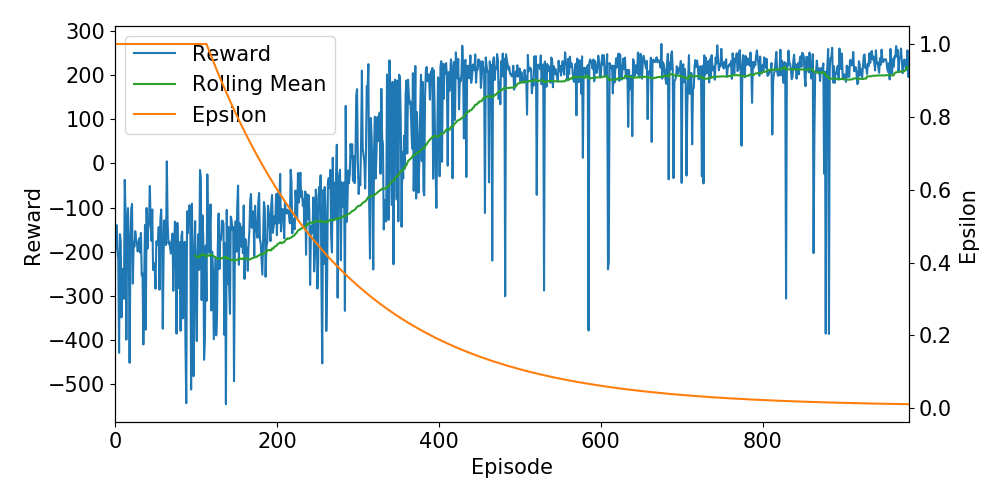
\includegraphics[width=\linewidth]{../logs/train_param_0059.png}
      \caption{}
  \label{fig:train_param_0059}
  \end{subfigure}
  \begin{subfigure}[b]{0.49\linewidth}
  \centering
  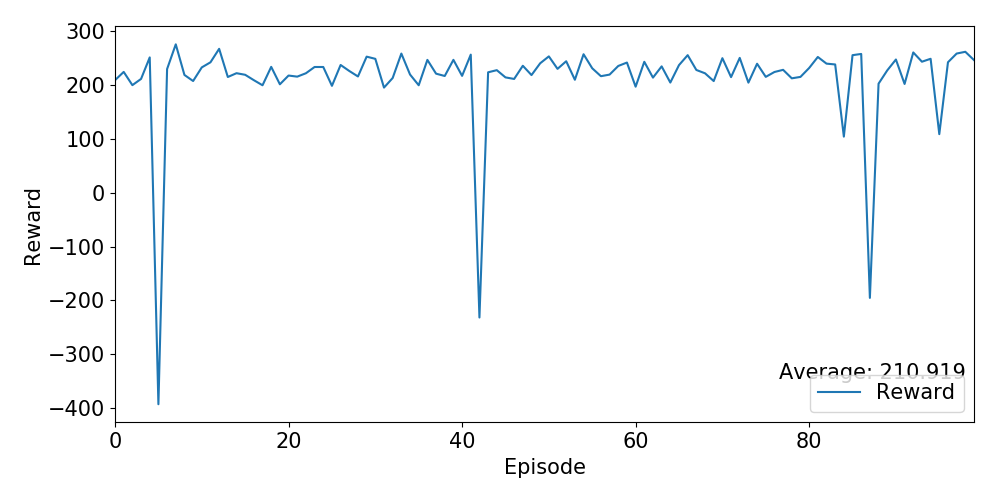
\includegraphics[width=\linewidth]{../logs/test_param_0059.png}
      \caption{}
  \label{fig:test_param_0059}
  \end{subfigure}
  \begin{subfigure}[b]{0.49\linewidth}
  \centering
  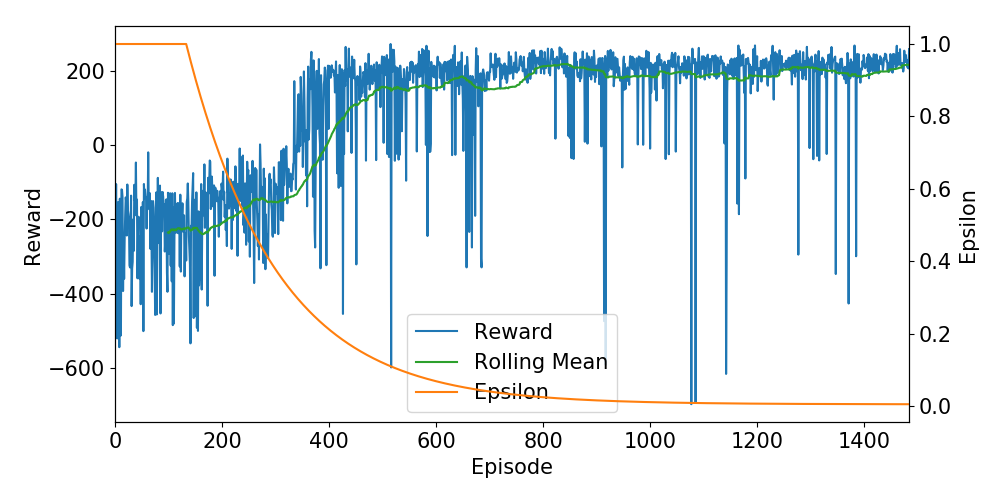
\includegraphics[width=\linewidth]{../logs/train_param_0060.png}
      \caption{}
  \label{fig:train_param_0060}
  \end{subfigure}
  \begin{subfigure}[b]{0.49\linewidth}
  \centering
  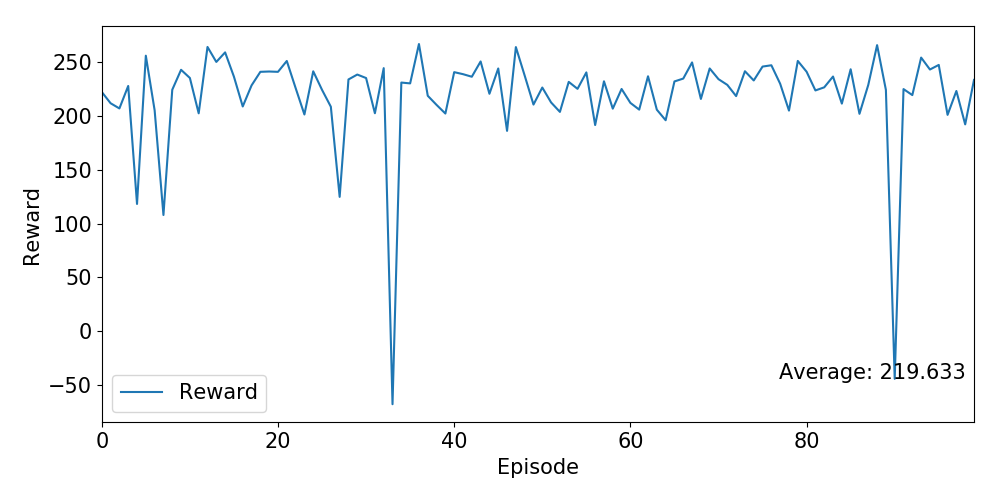
\includegraphics[width=\linewidth]{../logs/test_param_0060.png}
      \caption{}
  \label{fig:test_param_0060}
  \end{subfigure}
  \caption{DQN with "soft update" ($\tau=0.01$): learning curve (a) and testing result (b); and ($\tau=0.05$): learning curve (c) and testing result (d)}
  \label{fig:param_00590060}
\end{figure}

%%%%%%%%%%%%%%%%%%% figure here ^

\subsection{Experiment 3} \label{experiment3}
Some preliminary tests were run using Double DQN (DDQN) algorithm\cite{vanHasseltDeepReinforcementLearning2015}, in which Q value of the target network is chosen by the eval network: $Q_{\text{target}}=r+\gamma Q(S',\argmax_{a'}Q(S',a';\theta);\theta^-)$, instead of $Q_{\text{target}}=r+\gamma \max_{a'}(Q(S',a';\theta^-))$. The rest of the algorithm is identical to DQN, either with fixed Q-targets or "soft update". DDQN is supposed to be able to further stabilize the learning by preventing the two networks from drifting away from each other. However, I ran out of time searching for the ideal hyperparameter combinations for DDQN on LunarLander-v2. Here are the results: for DDQN with fixed Q-targets, the agent does not to be able to learn at all (shown in \textbf{Fig} \ref{fig:train_param_0083} and \ref{fig:train_param_0084}); for DDQN with soft update, the learning curve seems to converges to some sub-optimal value, with huge variances (shown in \textbf{Fig} \ref{fig:train_param_0077} and \ref{fig:train_param_0079}).

%%%%%%%%%%%%%%%%%%%figure here v
\begin{figure}[H]
  \centering
  \begin{subfigure}[b]{0.49\linewidth}
  \centering
  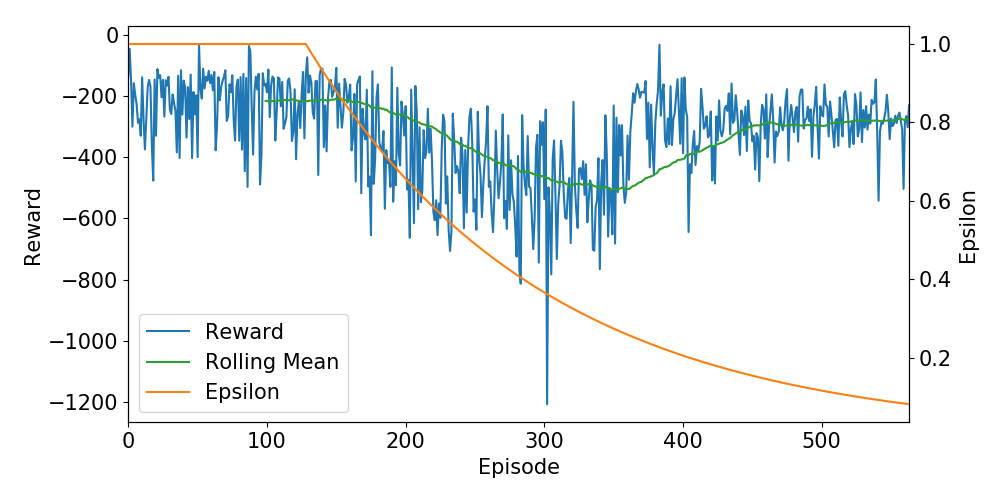
\includegraphics[width=\linewidth]{../logs/train_param_0083.png}
      \caption{}
  \label{fig:train_param_0083}
  \end{subfigure}
  \begin{subfigure}[b]{0.49\linewidth}
  \centering
  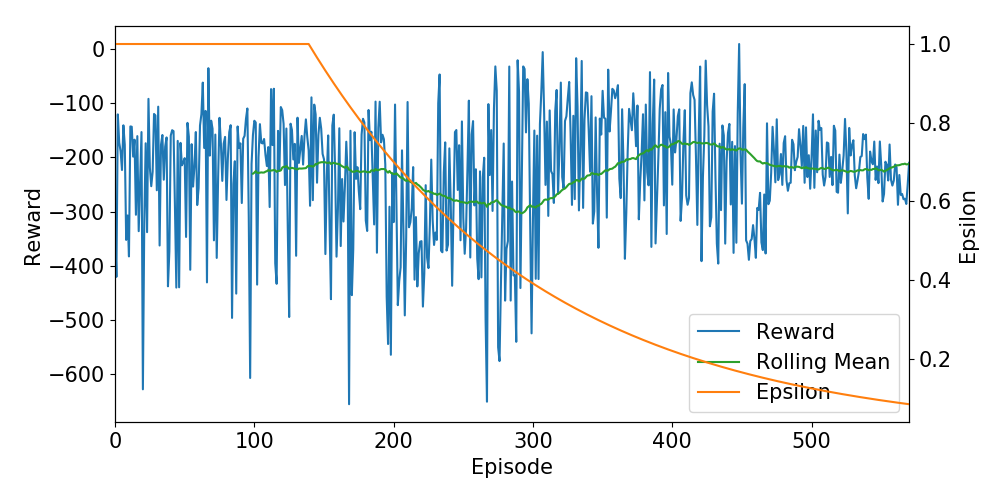
\includegraphics[width=\linewidth]{../logs/train_param_0084.png}
      \caption{}
  \label{fig:train_param_0084}
  \end{subfigure}
    \caption{DDQN with fixed Q targets (update interval: 500) at $\alpha=5\times 10^{-4}$ (a), and $\alpha=5\times 10^{-2}$ (b).}
  \label{fig:nnbestparam}
\end{figure}
  
  
\begin{figure}[H]
  \centering
   \begin{subfigure}[b]{0.49\linewidth}
  \centering
  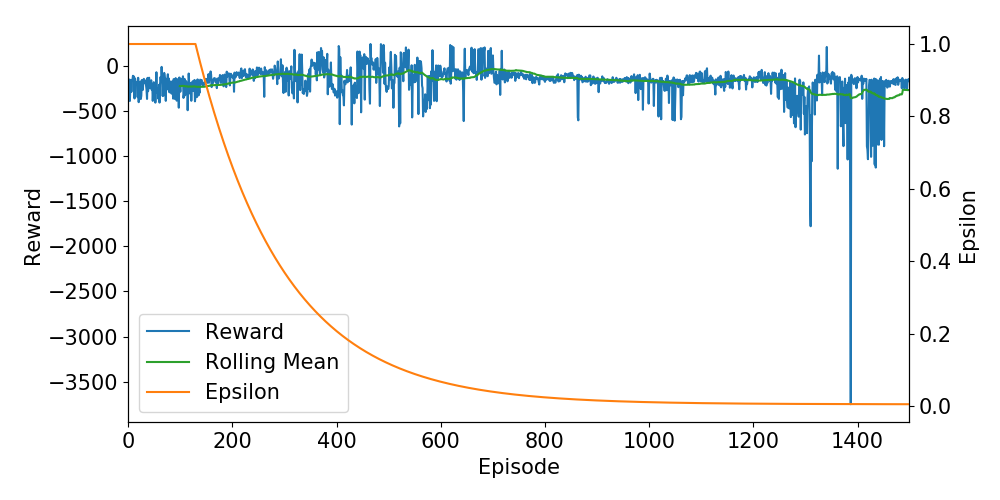
\includegraphics[width=\linewidth]{../logs/train_param_0077.png}
      \caption{}
  \label{fig:train_param_0077}
  \end{subfigure}
  \begin{subfigure}[b]{0.49\linewidth}
  \centering
  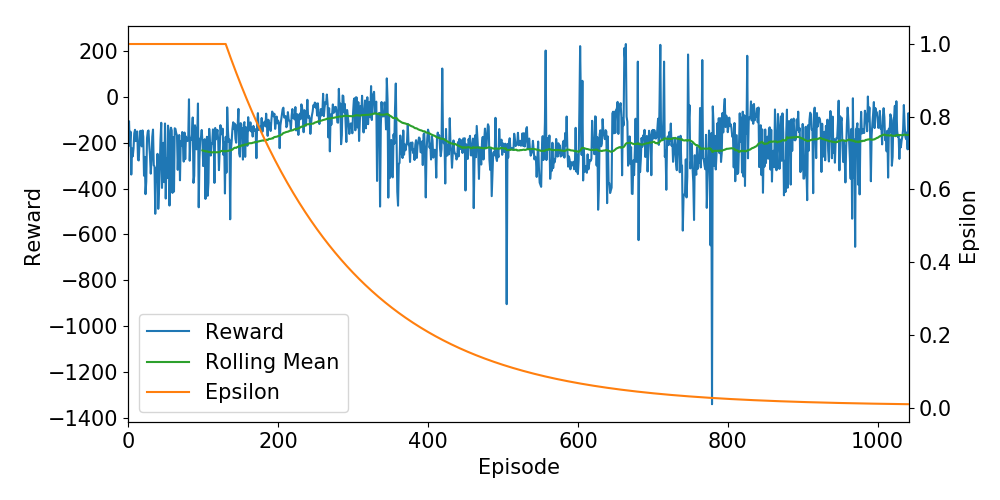
\includegraphics[width=\linewidth]{../logs/train_param_0079.png}
      \caption{}
  \label{fig:train_param_0079}
  \end{subfigure}
  \caption{DDQN with soft update ($\alpha=5\times 10^{-4}$) at $\tau=0.05$ (c), and $\tau=0.02$ (d).}
  \label{fig:nnbestparam}
\end{figure}

%%%%%%%%%%%%%%%%%%% figure here ^




\section{Difficulties} \label{difficulties}

   	\begin{itemize}
     		\item  DQN with fixed Q-targets
     			\begin{itemize}
					\item Extremely large continuous hyperparameter space.
       				\item Extremely high dimensional hyperparameter space.
					\item No intuition or theoretical support on the range of hyperparameters. I ended up using a grid search script to cover very large space
					\item Ambiguity in algorithmic specifics and naming conventions: is fixed Q targets and memory replay considered part of a "bare-bone" DQN, etc.
    			 \end{itemize}
		     \item  DQN with soft update
    			 \begin{itemize}
    				   \item Introduced yet another hyperparameter $\tau$ to tune.
				 \end{itemize}
			\item  DDQN
    			 \begin{itemize}
    				   \item Introduced yet another hyperparameter (a boolean to control if DDQN is used) to tune, making the totally number of parameters up to 20.
				       \item Again, the lack of intuition or theoretical support on the range of hyperparameters makes it extremely difficult to find a successful combination of hyperparameters.
				       \item If I had more time, I would like to search for hyperparameter combinations for DDQN and run tests to see if it is indeed able to stabilize learning process.
       				   
     			 \end{itemize}
	\end{itemize}




%%%%%%%%%%%%%%%%%%%%%%figure here v
%%%%%%%%%%%%%%%%%%%%%%figure here ^


%\section{Appendix} \label{appendix}
%Code used to run experiments described in this report is hosted here: \burl{https://github.gatech.edu/rchen350/cs7642summer2018p1}. 

\bibliographystyle{unsrt}
\bibliography{ref}

\end{document}
















